%!TEX root = ../thesis.tex

\chapter{Introduction}

\graphicspath{{Figs}}

\section{Edge computing}

Edge computing is a newer computation paradigm as compared to cloud computing.
The difference between them is that edge computing brings computation closer to the
edge of the network. As more of the data is being generated near the edge of the
network, edge computing enables the data to be processed near the data source.
\cite{weisongshiEdgeComputingVision2016}

\subsection{Why use edge computing in place of cloud computing?}

The most important reason for using edge computing is that it reduces the
latency as the data has to travel a shorter distance.
\cite{weisongshiEdgeComputingVision2016} In addition to this, with the emergence of
Internet of Things, the data generated at the edge is expected to grow rapidly.
For example, it is expected that the autonomous vehicles will generate data in
the order of 1Tb per second. In such a case, it may not be possible for the
cloud to keep pace with the data generated at the edge. Edge computing can help
in this situation as it can process the data at the edge itself.

\subsection{Challenges with edge computing}

One of the major challenges with edge computing is that the edge devices are
resource constrained. They have limited processing power, memory and storage.
Often, this problem is solving using offloading. A node that is low on resources
may enlist the other nodes for help. For example, if a node is low on storage
space, then the data generated on this node or the data this node was supported
to store may be offloaded to other nodes in the network. Similarly, data
processing can be offloaded to other nodes.

The other challenge is that, no node in the edge network has complete knowledge of
the edge network. This is in contrast with cloud computing where a central node is
responsible for all the processing and does not need to coordinator with others.
As such, it can become difficult to do any computation on the edge as the nodes
may not be having all the information required for the computation.

\subsection{Edge computing for vehicles}

Researchers have been working on using edge computing for vehicles for a while
now. In autonomous vehicles, the decision must be taken quickly as there is very
low tolerance for latency. Further, the data that a vehicle generate is rarely
needed outside the geographical vicinity in which the vehicle is present. Using
edge computing makes the common use-case faster. As such, edge computing can be
used to improve the performance of the autonomous vehicles.

\begin{figure}[h]
      \centering
      \includegraphics[width=1.0\textwidth]{"Vehicular Edge Network.png"}
      \caption{Vehicular edge network architecture}
\end{figure}

Vehicular edge networks usually consists of a central cloud to which a number of
gateway devices called roadside units (RSUs) are connected. The RSUs are further
connected to the vehicles. Vehicular edge networks are highly dynamic and
vehicles change their position quite often. Because of this, hand-offs may be
needed very frequently.

\section{Problem statement}

Because of the issues described above, we need to have some kind of method to
enable nodes to find out where the required data may be present in the edge
network.

We are trying to come up with a method for answering resource queries in edge
networks while keeping in mind the constraints on resources that come with edge
computing.

Requirements for the solution:
\begin{itemize}
      \item Data privacy is maintained and the data itself should not be used
            for indexing or querying
      \item The solution should be scalable
      \item The algorithm should preferably be online -- it should be able to
            index or answer queries for the data that is being generated
\end{itemize}

Further, it is not possible to simply boardcast the query to all the nodes in
the network, as it would very inefficient. Doing so will lead to privacy issues, as
the queries would be known to every node in the network. Also, caching the data
on other nodes should be avoided because of the privacy issues.

\subsubsection{Use cases}

The problem of resource or data discovery is by no mean unique to edge computing
or IoT. Even in the computer architecture, Flat Cache-Only Memory Architecture
(COMA) faces the similar problem. In Flat COMA, memory lines can freely migrate.
Whenever there is a cache miss, the memory line must be located in the network and
migrated to where it is needed.
\cite{joseptorrellasCacheOnlyMemoryArchitecture}

But in our work, we are trying to solve this problem in the context of edge
computing, where the nodes may be static or dynamic. Weather crowd-sensing would
need only static nodes, but in vehicular edge networks, the nodes are dynamic.


\chapter{Literature review}

Numerous surveys have been done on edge computing as well as data access in IoT
or distributed systems. These include surveys by \citet{kouahlaSurveyBigIoT2022} and
\citet{fathyLargeScaleIndexingDiscovery2018}.

\citet{fathyLargeScaleIndexingDiscovery2018} prescribes the following taxonomy
for queries in IoT:

\begin{itemize}
      \item \textbf{Data queries}: Here, we are only interested in the data,
            regardless of its source. They may be indexed by:
            \begin{itemize}
                  \item Spatial features: The data may be indexed using spatial
                        attributes, e.g. geo-coordinates. Space filling curves
                        may be used to reduce dimensionality.
                  \item Thematic features: data is indexed based on the keywords
                        or its attributes.
                  \item Temporal features: data is indexed based on the time at
                        which it was generated.
            \end{itemize}

      \item \textbf{Resource queries}: Rather than finding the data stored on
            the node, the nodes are only interested in finding a physical
            resource on the network.
      \item \textbf{Higher-level abstractions}: the queries are based on
            higher-level abstractions like events, activities and patterns which
            require data from several nodes to be combined and processed.
\end{itemize}

\citet{kouahlaSurveyBigIoT2022} also classifies indexing techniques as below:

\begin{itemize}
      \item Indexing structures in a Multidimensional Space
            \begin{itemize}
                  \item Hashing-based techniques
                  \item Tree-based techniques
                  \item Bitmap-based techniques
            \end{itemize}
      \item Indexing structures in a Metric Space
            \begin{itemize}
                  \item Tree-based techniques
            \end{itemize}
\end{itemize}

In this work, the focus is on resource queries. The advantage of focusing on
resource queries over data queries is that the data queries can be trivially
answered once the resource queries are answered. Further, it allows the nodes to
implement some kind of authentication mechanism to ensure that the data is not
publically available.


In 2012, \citet{federicapaganelliDHTBasedDiscoveryService2012} proposed a scheme
that used DHTs for service discovery in Internet of Things. Their method allowed
multi-attribute queries as well as range queries. The method consists of three
layers. They first used a space-filling curve to linearize and map the
multidimensional domain into a one-dimensional one. Then a Prefix-Hash Table is
used on top of a generic DHT with standard interface for get and put. At the
end, the DHT is an implementation based on the Kademlia algorithm.
\citet{federicapaganelliDHTBasedDiscoveryService2012}, however, did not apply
DHTs to edge networks.

Researchers have also attempted to use Gaussian Mixture Models (GMM) for
searching and indexing in edge computing.


\section{Distributed Hash Tables}

The Distributed Hash Tables (DHTs) are similar to the conventional hash tables,
except that the key-value pairs are stored across multiple nodes in the network.
Distributed hash tables are highly scalable and fault-tolerant. Like traditional
hash-tables, DHTs also support ``get'' and ``put'' operations. They are commonly
used in the peer-to-peer networks. There exist multiple variants of DHTs
including Chord \cite{ChordScalablePeertopeer}, Tapestry
\cite{zhaoTapestryResilientGlobalscale2004} and Kademlia
\cite{petarmaymounkovKademliaPeertoPeerInformation2002}.

In DHTs, the data is placed deterministically on the nodes in the network. DHTs
are self-organizing and self-healing.

Of these DHTs, Kademlia is the most widely used. It is used in BitTorrent
\cite{andrewloewensternDHTProtocol2008} as well as in Ethereum. Every key-value
pair is stored with multiple nodes in the network. This is done to ensure that
the network is robust to node failures. Kademlia is not affected if a node
leaves or joins the network. Each node joining the Kademlia randomly generates a
160-bit identifier.
\cite{petarmaymounkovKademliaPeertoPeerInformation2002}

\subsection{How does Kademlia work?}

Whenever a key-value pair is to be stored in the network, a 160 bit hash of the
key is calculated. Then, nodes with the identifier closest to the hash are
selected for storing the key-value pair. For measuring the distance and finding
the closest nodes to a given key, Kademlia uses XOR metric. Even though it is
non-euclidean, the XOR metric satisfies all four properties of a distance
metric.
\cite{MetricSpace2022}

Similarly, when finding the value for a given key, the nodes with the identifier
closest to the hash of the key are selected. An attempt is then made to retrieve
the corresponding values from these nodes.

The authors also propose an XOR based routing algorithm for finding the node
with the identifier closest to a given key. With the algorithm proposed, in each
iteration, we get one bit closer to the target node. Thus, if the network size
if $n$, then the algorithm takes $O(log(n))$ iterations to find the target node.

Nodes in Kademlia can be visualized as leaves in a binary tree, where the position of
each of the nodes is given by its identifier. In the algorithm, each node is
required to maintain a routing table. Each of the node is expected to store
information about $k$ nodes from each of the maximal tree which it is not
a part of in its routing table. The information includes the identifier, IP address
and the port number. The requirement of storing information about $k$ nodes from
each is to bring redundancy and to ensure that the network is robust to node
failures.

\begin{figure}[h]
      \centering
      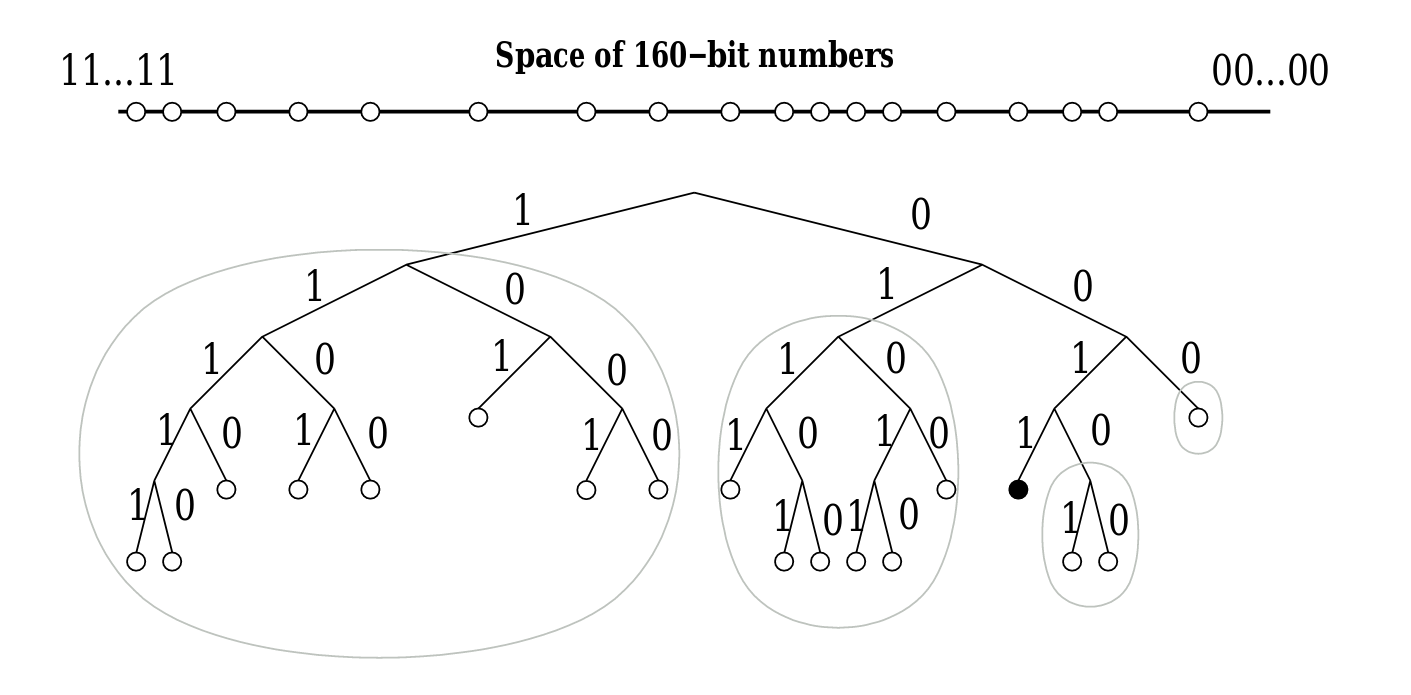
\includegraphics[width=1.0\textwidth]{kademlia.png}
      \caption[Kademlia]{The node with identifier 0011 stores information about
            nodes in four subtrees, which are encircled.
            \cite{petarmaymounkovKademliaPeertoPeerInformation2002}}
      % \caption[Routing in Kademlia]
\end{figure}

\section{Learned indexes}

\citet{kraska2018} proposed that machine learning models may be used along with
traditional data structures to improve performance. For example, in a sorted
array, instead of using binary search or an index, a machine learning model may
be used to predict the appropriate index of the element. This can be applied to
many structures like B-trees, bloom filters, etc.

Several learned indexes have been proposed -- Learned Spatial Index
\cite{pandeyCaseLearnedSpatial2020} for answering spatial range queries, Learned
Secondary Index \cite{kipfLSILearnedSecondary2022} for unsorted data,
RadixSpline \cite{kipfRadixSplineSinglePassLearned2020}, an index that can be
built in a single pass and Practical Learned Index (PLEX)
\cite{stoianPracticalLearnedIndexing2021} which was introduced to make the
learned index more practical by reducing the number of hyperparameters to just
one.

Learned indices have recently been gaining popularity in the database community
recently. The idea of using machine learning models has been so influential that
researchers are applying the same approach to even the sorting algorithms.
\cite{kristoCaseLearnedSorting2020}

\citet{kraska2018} also proposed a Recursive Model Index which is hierarchical
in nature. They are similar to B-trees except, a machine learning model is used
in each stage. In each stage, the model predicts another model until the leaf
node is reached where the data is stored. It can also be viewed as each node
picking a better expert to answer the query.

\begin{figure}[h]
      \centering
      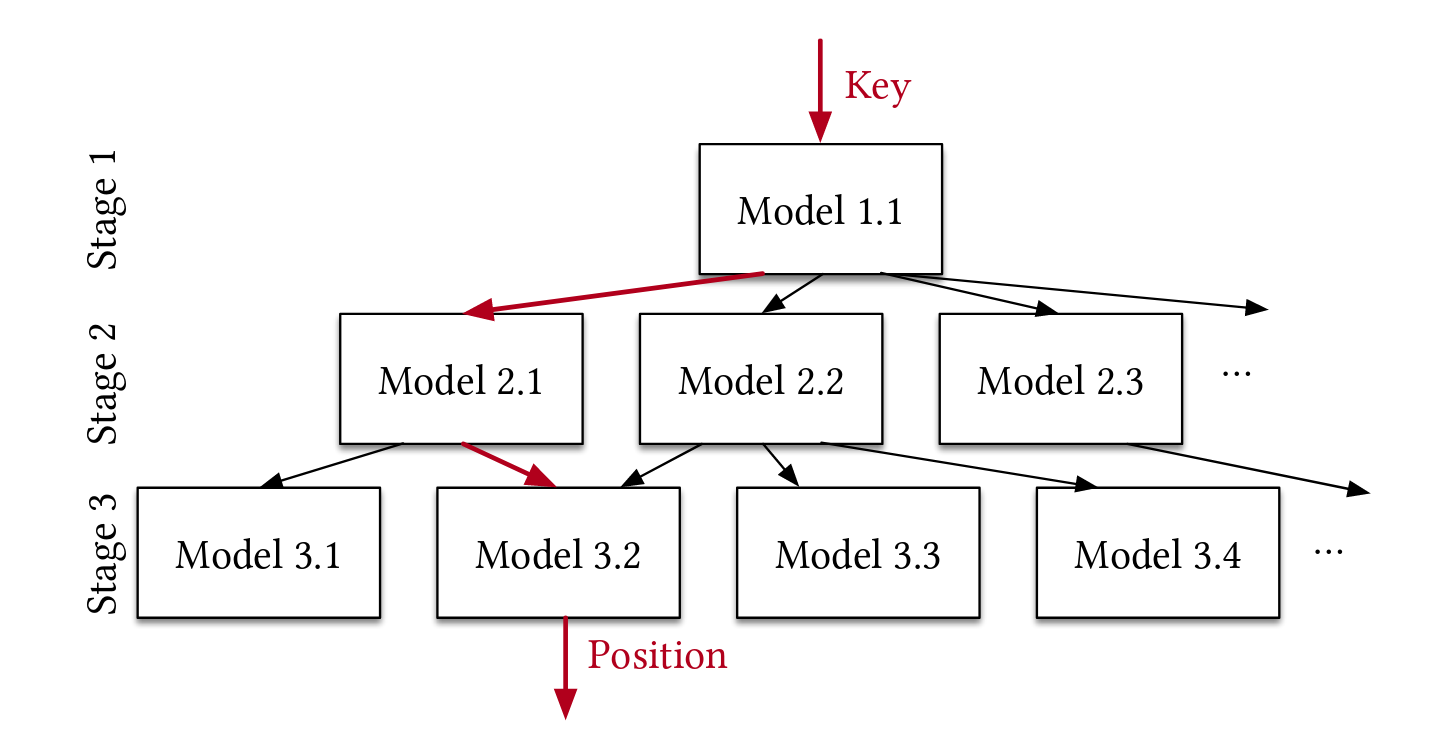
\includegraphics[width=1.0\textwidth]{RMI.png}
      \caption[Recursive Model Index]{The Recursive Model Index.
            \cite{kraska2018}}
\end{figure}
\chapter{Proposed Methodology}

\section{Using Distributed Hash Tables for Edge Computing}

We tried to extend DHTs and learned indices to edge networks. We intend to use
Kademlia not for content discovery, but only the XOR based routing algorithm
proposed by \citet{petarmaymounkovKademliaPeertoPeerInformation2002} for
routing, once the target node is determined using the learned index.

\citet{xieEfficientIndexingMechanism2019} observed that DHTs may use a longer
path than the shortest possible path between two nodes. This happens because the
nodes which may be logically close to each as determined by XOR metric on node
identifier may, in fact, be far apart physically. One possible way of solving
this problem is to modify the node identifier used by Kademlia so that it is
based on the location of the node. \citet{mengweiImprovementKademliaBased2013}
did this by using the IP address of the nodes as the prefix in the node
identifier. While this should make the routing in Kademlia more efficient, this
method suffers from the drawback that the IP address of the node may change.

The another way in which node identifiers can be modified is to encode the
services offered by a node into its identifier. For example, if a node is offering
weather sensing service, its identifier may be prefixed by ``10'' or if it is
offering road-traffic information, its identifier may be prefixed by ``01''.
Similarly, if both the services are offered by the node, its identifier may
start with ``11''. Because of how routing works in Kademlia, it would be trivial
to search for nodes offering a particular service if this scheme is used. While
we could not find any work that has done this, we believe that this too will
have limitations.

We used an open-source Python library to test if Kademlia would be
appropriate for this use case. \cite{KademliaIndexRst}

\section{Using Learned Indices for Edge Computing}

While \citet{kraska2018} proposed that the model should be trained only once, we
believe it would be better if the model is updated periodically so that it can
serve the queries better.

To test the performance of learned indexes, we simulated an edge network using
Python. Inside each edge node, we put five key value pairs. The keys were
randomly generated strings and the values were randomly generated integers.
First, keys were encoded using ordinal encoding. Then a one-vs-rest multi-class
classifier was used to predict the location in which the key-value pairs might be
stored. Though the results were not conclusive, using a real world dataset by
\citet{taxi&limousinecommissionNewYorkTaxi} should give conclusive results. This
is because random data carrier the most amount of entropy, it is the most
difficult to compress, and real world data usually has a lot of redundancy and
patterns which the model can learn.

\section{Conclusion}

We believe learned indexes can be a good fit for this problem. Along with
learned indexes, the routing algorithm proposed in Kademlia can be used to
routing after modifying it so that it favors the shortest path between the nodes
based on the scheme proposed by \citet{mengweiImprovementKademliaBased2013}.